% SC 2026 Submission
% ML+LLM Hybrid for HPC I/O Bottleneck Detection
%
% Format: IEEE proceedings (10 pages excl. bibliography)
% Template: IEEEtran.cls (IEEE Conference)

\documentclass[conference]{IEEEtran}

% --- Packages ---
\usepackage{cite}
\usepackage{amsmath,amssymb,amsfonts}
\usepackage{algorithmic}
\usepackage{graphicx}
\usepackage{textcomp}
\usepackage{xcolor}
\usepackage{booktabs}       % Professional tables
\usepackage{multirow}
\usepackage{hyperref}
\usepackage{subcaption}     % Sub-figures
% \usepackage{balance}     % Balance final page columns (install if needed)

% --- Figure paths ---
\graphicspath{{figures/}{figures/preprocessing/}{figures/eda/}}

% --- Hyperref setup ---
\hypersetup{
    colorlinks=true,
    linkcolor=black,
    citecolor=black,
    urlcolor=blue,
    pdfauthor={},            % Double-anonymous: no author info
    pdftitle={ML+LLM Hybrid for HPC I/O Bottleneck Detection},
}

% --- Custom commands ---
\newcommand{\system}{IOSage}              % System name (placeholder)
\newcommand{\dataset}{Polaris-IO}          % Dataset name
\newcommand{\ie}{i.e.,\xspace}
\newcommand{\eg}{e.g.,\xspace}
\newcommand{\etal}{et~al.\xspace}

% Double-anonymous: suppress author info
\def\BibTeX{{\rm B\kern-.05em{\sc i\kern-.025em b}\kern-.08em
    T\kern-.1667em\lower.7ex\hbox{E}\kern-.125emX}}

\begin{document}

% =====================================================================
% Title
% =====================================================================
\title{ML+LLM Hybrid for I/O Bottleneck Detection and \\
Code-Level Recommendation in HPC Systems}

% Double-anonymous: no authors
\author{}

\maketitle

% =====================================================================
% Abstract
% =====================================================================
\begin{abstract}
% TODO: Write abstract (250 words max)
% Structure: Problem -> Gap -> Approach -> Results -> Impact
\end{abstract}

% =====================================================================
% 1. Introduction
% =====================================================================
\section{Introduction}
\label{sec:intro}

% TODO: 1.5 pages
% - Problem: I/O bottlenecks in HPC, gap between detection and actionable fixes
% - Existing approaches and their limitations (AIIO, Drishti, IOAgent, WisIO)
% - Our approach: ML+LLM hybrid with benchmark-grounded KB
% - Contributions (3-4 bullet points)

% Placeholder text with citations to validate bibliography pipeline
Prior work on I/O bottleneck detection includes rule-based systems~\cite{bez2022drishti, devarajan2025wisio},
ML classifiers~\cite{dong2023aiio}, and LLM-based approaches~\cite{zheng2025ioagent, lockwood2024ion}.

% =====================================================================
% 2. Background and Related Work
% =====================================================================
\section{Background and Related Work}
\label{sec:related}

% TODO: 1.5 pages
% - Darshan I/O instrumentation
% - ML-based I/O analysis (AIIO, WisIO)
% - LLM-based approaches (IOAgent, ION)
% - ML+LLM integration patterns in systems (RCACopilot, etc.)

% =====================================================================
% 3. System Design
% =====================================================================
\section{System Design}
\label{sec:design}

% TODO: 2 pages
% - Architecture overview figure
% - Phase A: Benchmark execution + KB construction
% - Phase B: ML classifier training (gold + silver labels)
% - Phase C: Online inference (ML -> SHAP -> RAG -> LLM)

% =====================================================================
% 4. Dataset and Preprocessing
% =====================================================================
\section{Dataset and Preprocessing}
\label{sec:dataset}

% TODO: 1.5 pages
% Use figures from paper/figures/preprocessing/
% Use tables from paper/tables/

\subsection{Dataset}
\label{sec:dataset:data}

% Table: Dataset summary
\begin{table}[t]
\centering
\caption{Dataset Summary}
\label{tab:dataset}
\begin{tabular}{lr}
\toprule
\textbf{Property} & \textbf{Value} \\
\midrule
Source system & ALCF Polaris \\
Collection period & Apr 2024 -- Feb 2026 \\
Raw Darshan logs & 1,397,216 \\
After cleaning & 131,151 \\
Retention rate & 9.4\% \\
Total features & 186 \\
\midrule
\multicolumn{2}{l}{\textit{Feature breakdown:}} \\
~~Raw counters & 136 \\
~~Indicators & 8 \\
~~Derived ratios & 40 \\
~~Metadata & 2 \\
\midrule
Train / Val / Test & 91,807 / 19,672 / 19,672 \\
Split method & Temporal (70/15/15) \\
\bottomrule
\end{tabular}
\end{table}

\subsection{Feature Extraction}
\label{sec:dataset:features}

% 186 raw features -> 157 ML-ready after exclusion

\subsection{Preprocessing Pipeline}
\label{sec:dataset:preprocessing}

% Cleaning, engineering, normalization
% Figure: Data characterization (3 panels)
% \begin{figure}[t]
%   \centering
%   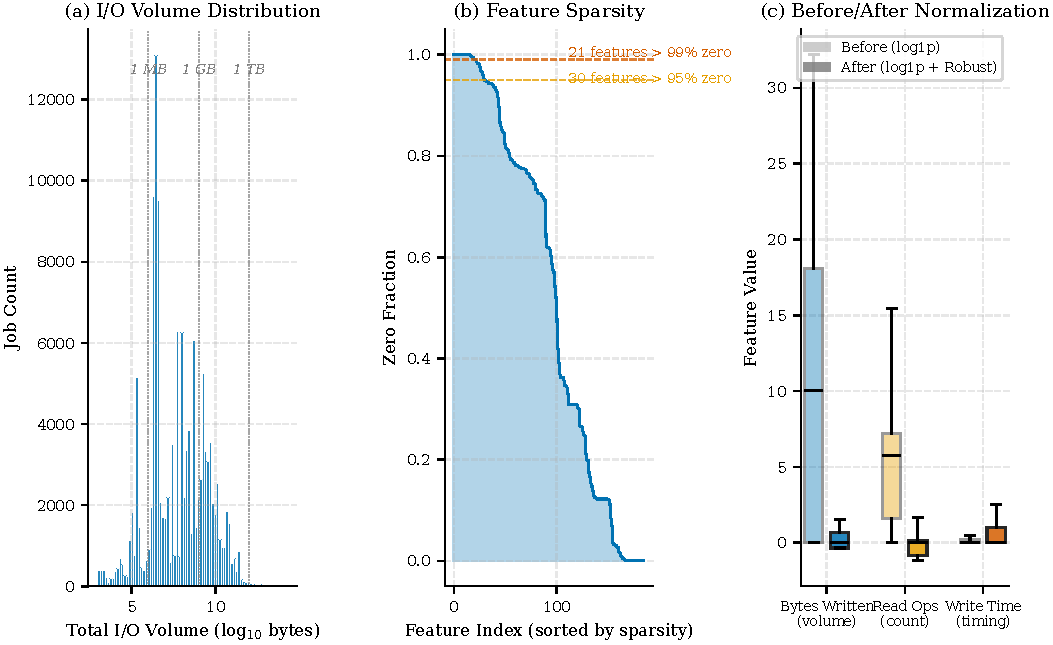
\includegraphics[width=\columnwidth]{fig_data_characterization.pdf}
%   \caption{Dataset characterization: (a) I/O volume distribution,
%   (b) feature sparsity, (c) normalization effect.}
%   \label{fig:data_char}
% \end{figure}

% Table: Normalization methods
\begin{table}[t]
\centering
\caption{Group-Specific Normalization Strategy}
\label{tab:normalization}
\begin{tabular}{lrl}
\toprule
\textbf{Feature Group} & \textbf{\#} & \textbf{Method} \\
\midrule
    Volume & 12 & $\log(1{+}x)$ + RobustScaler \\
    Count & 39 & $\log(1{+}x)$ + RobustScaler \\
    Histogram & 20 & $\log(1{+}x)$ \\
    Top4 & 24 & $\log(1{+}x)$ \\
    Timing & 25 & $\log(1{+}x)$ + RobustScaler \\
    Ratio Unbounded & 14 & $\log(1{+}x)$ \\
    Derived Absolute & 3 & $\log(1{+}x)$ \\
    Metadata & 2 & $\log(1{+}x)$ \\
    Conditional Size & 2 & $\log(1{+}x)$ \\
    Ratio & 23 & none \\
    Indicator & 8 & none \\
    Timestamp & 8 & none \\
    Categorical & 4 & none \\
    Rank Id & 2 & none \\
\bottomrule
\end{tabular}
\end{table}

\subsection{Temporal Data Split}
\label{sec:dataset:split}

% 70/15/15 temporal split justification
% Figure: Temporal split
% \begin{figure}[t]
%   \centering
%   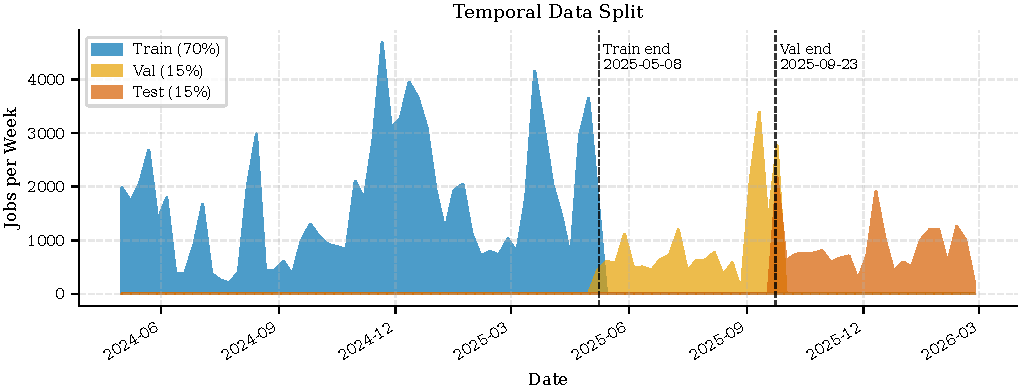
\includegraphics[width=\columnwidth]{fig_temporal_split.pdf}
%   \caption{Temporal train/val/test split.}
%   \label{fig:temporal_split}
% \end{figure}

% =====================================================================
% 5. Methodology
% =====================================================================
\section{Methodology}
\label{sec:method}

% TODO: 2 pages
\subsection{Bottleneck Taxonomy}
\label{sec:method:taxonomy}

\subsection{ML Classifier}
\label{sec:method:ml}

\subsection{SHAP Attribution}
\label{sec:method:shap}

\subsection{LLM Recommendation Engine}
\label{sec:method:llm}

% =====================================================================
% 6. Evaluation
% =====================================================================
\section{Evaluation}
\label{sec:eval}

% TODO: 2 pages
\subsection{Experimental Setup}
\label{sec:eval:setup}

\subsection{Detection Performance}
\label{sec:eval:detection}

\subsection{Recommendation Quality}
\label{sec:eval:recs}

\subsection{Ablation Study}
\label{sec:eval:ablation}

\subsection{Case Studies}
\label{sec:eval:cases}

% =====================================================================
% 7. Discussion
% =====================================================================
\section{Discussion}
\label{sec:discussion}

% TODO: 0.5 pages
% Limitations, threats to validity, future work

% =====================================================================
% 8. Conclusion
% =====================================================================
\section{Conclusion}
\label{sec:conclusion}

% TODO: 0.5 pages

% =====================================================================
% Acknowledgments (only in camera-ready, not submission)
% =====================================================================
% \section*{Acknowledgments}
% This research used resources of the Argonne Leadership Computing Facility...

% =====================================================================
% References
% =====================================================================
\bibliographystyle{IEEEtran}
\bibliography{references}

\end{document}
